\section{TASK 5, Constructing bifurcation diagrams}

\begin{frame}
	\frametitle{Euler's method -- Andronov-Hopf system}
	\paragraph{Data}\vspace{-4mm}
	\begin{figure}[H]
		\subfloat{
			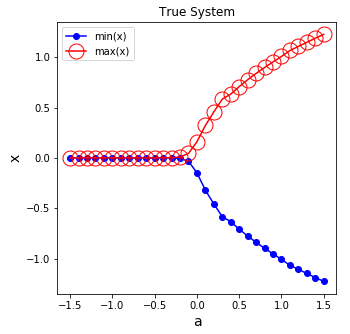
\includegraphics[width=.28\linewidth]{figures/euler/bifurcation/true_and_hopf_x.png}
		}\quad
		\subfloat{
			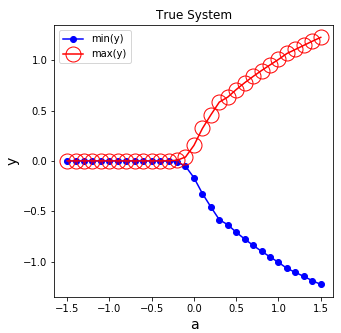
\includegraphics[width=.28\linewidth]{figures/euler/bifurcation/true_and_hopf_y.png}
		}
	\end{figure}
	\paragraph{Approximation}\vspace{-4mm}
	\begin{figure}[H]
		\subfloat{
			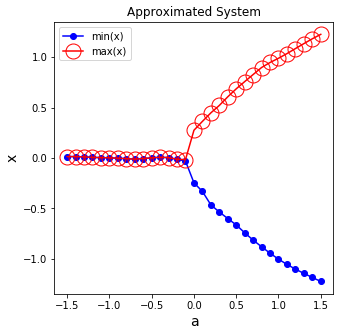
\includegraphics[width=.28\linewidth]{figures/euler/bifurcation/approx_and_hopf_x.png}
		}\quad
		\subfloat{
			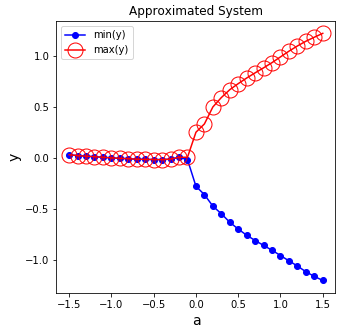
\includegraphics[width=.28\linewidth]{figures/euler/bifurcation/approx_and_hopf_y.png}
		}
	\end{figure}
\end{frame}

\begin{frame}
	\frametitle{Euler's method -- R\"ossler attractor}
	\paragraph{Data}\vspace{-4mm}
	\begin{figure}[H]
		\subfloat{
			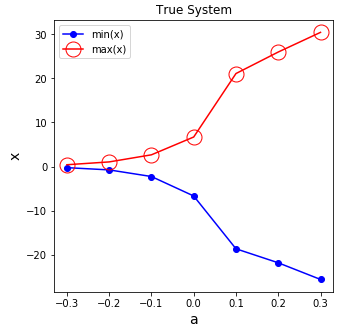
\includegraphics[width=.28\linewidth]{figures/euler/bifurcation/true_roe_x.png}
		}\quad
		\subfloat{
			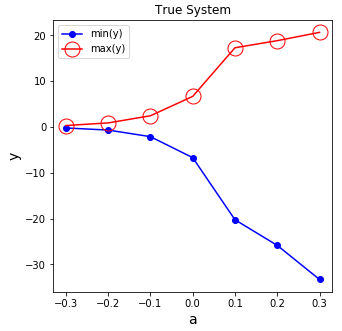
\includegraphics[width=.28\linewidth]{figures/euler/bifurcation/true_roe_y.png}
		}\quad
		\subfloat{
			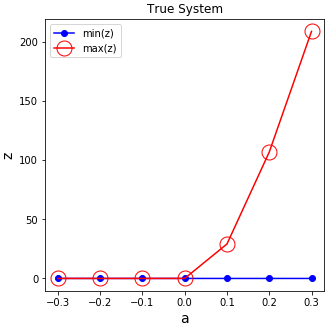
\includegraphics[width=.28\linewidth]{figures/euler/bifurcation/true_roe_z.png}
		}
	\end{figure}
	\paragraph{Approximation}\vspace{-4mm}
	\begin{figure}[H]
		\subfloat{
			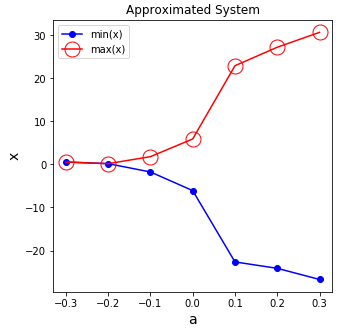
\includegraphics[width=.28\linewidth]{figures/euler/bifurcation/approx_roe_x.png}
		}\quad
		\subfloat{
			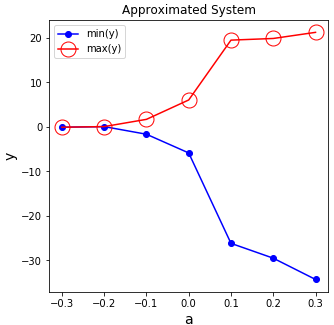
\includegraphics[width=.28\linewidth]{figures/euler/bifurcation/approx_roe_y.png}
		}\quad
		\subfloat{
			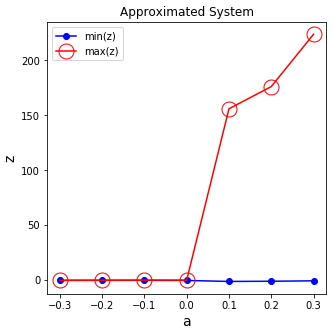
\includegraphics[width=.28\linewidth]{figures/euler/bifurcation/approx_roe_z.png}
		}
	\end{figure}
\end{frame}

\begin{frame}
\frametitle{Runge-Kutta method -- Andronov-Hopf system}
	\paragraph{Data}\vspace{-4mm}
	\begin{figure}[H]
		\subfloat{
			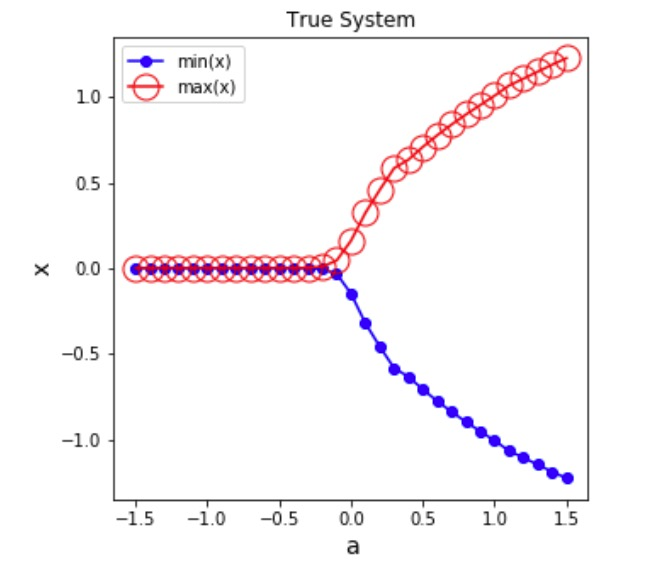
\includegraphics[width=.28\linewidth]{figures/runge_kutta/bifurcation/true_and_hopf_x.png}
		}\quad
		\subfloat{
			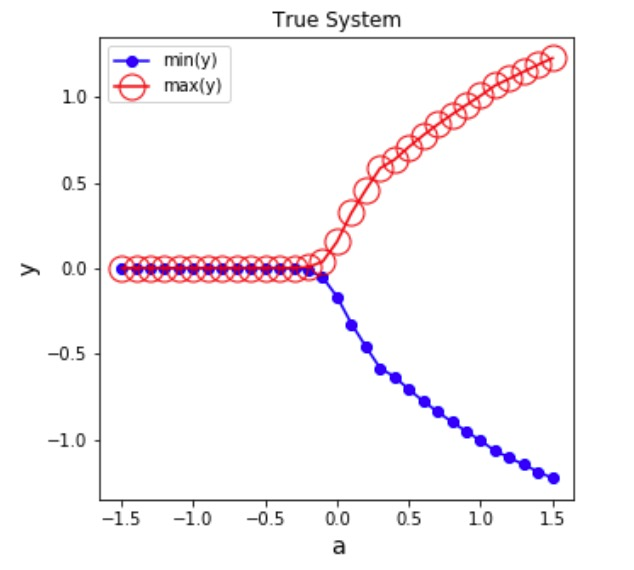
\includegraphics[width=.28\linewidth]{figures/runge_kutta/bifurcation/true_and_hopf_y.png}
		}
	\end{figure}
	\paragraph{Approximation}\vspace{-4mm}
	\begin{figure}[H]
		\subfloat{
			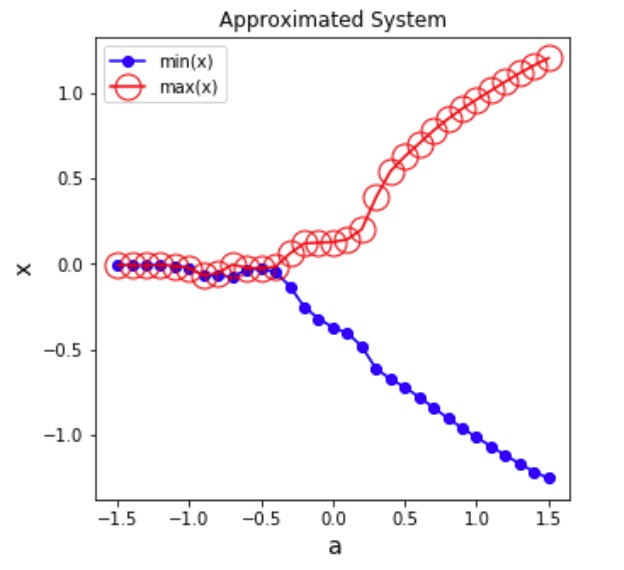
\includegraphics[width=.28\linewidth]{figures/runge_kutta/bifurcation/approx_and_hopf_x.png}
		}\quad
		\subfloat{
			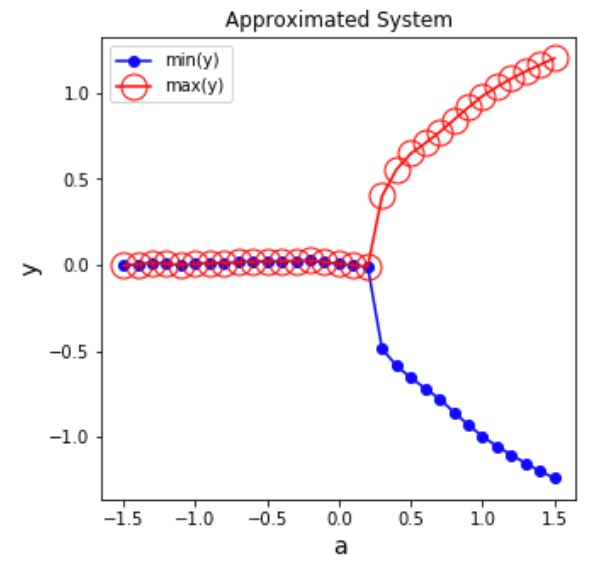
\includegraphics[width=.28\linewidth]{figures/runge_kutta/bifurcation/approx_and_hopf_y.png}
		}
	\end{figure}
\end{frame}

\begin{frame}
	\frametitle{Runge-Kutta method -- R\"ossler attractor}
	\paragraph{Data}\vspace{-4mm}
	\begin{figure}[H]
		\subfloat{
			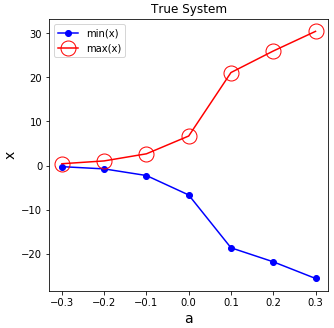
\includegraphics[width=.28\linewidth]{figures/runge_kutta/bifurcation/true_roe_x.png}
		}\quad
		\subfloat{
			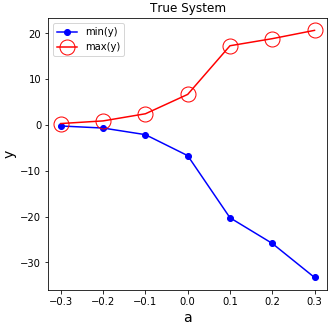
\includegraphics[width=.28\linewidth]{figures/runge_kutta/bifurcation/true_roe_y.png}
		}\quad
		\subfloat{
			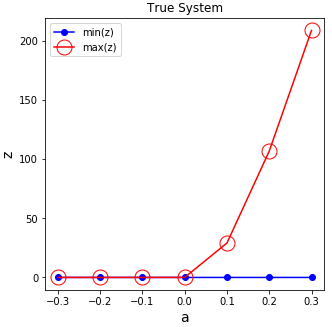
\includegraphics[width=.28\linewidth]{figures/runge_kutta/bifurcation/true_roe_z.png}
		}
	\end{figure}
	\paragraph{Approximation}\vspace{-4mm}
	\begin{figure}[H]
		\subfloat{
			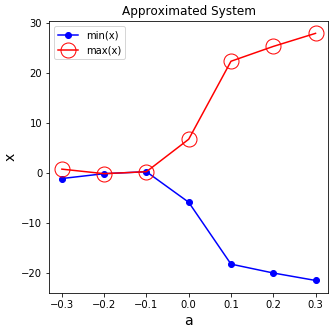
\includegraphics[width=.28\linewidth]{figures/runge_kutta/bifurcation/approx_roe_x.png}
		}\quad
		\subfloat{
			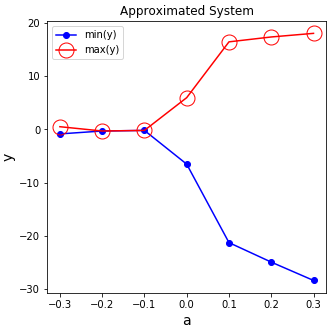
\includegraphics[width=.28\linewidth]{figures/runge_kutta/bifurcation/approx_roe_y.png}
		}\quad
		\subfloat{
			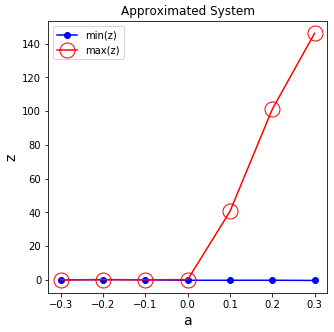
\includegraphics[width=.28\linewidth]{figures/runge_kutta/bifurcation/approx_roe_z.png}
		}
		\end{figure}
\end{frame}

